%I think the story here is that fears of the costs of library OSes are greatly exaggerated, and the performance is fine + it is easy to use.  Although SGX has a lot of limits, it doesn't have to be hard to bring up code on SGX (or other upcoming secure HW platforms) quickly.
%* Yes, you can do better with custom code in swift or whatever, but a lot of people benefit from thunking code down and having it "just work" with protection
%To this end, we also contribute usability enhancements, like dynamic linking, remote attestation, ipc, fork, etc.
%We contribute a measurement of a relatively mature SGX libos on real hardware.
%Shit works, lots of people are using Graphene.

\section{Intel SGX Overview}
\label{sec:sgx:overview}

This section summarizes SGX,
and current design points for running or porting applications on the SGX platform.
%and the legacy frameworks of porting 
%including \haven{}~\cite{baumann14haven}, \scone{}~\cite{osdi16scone}, and Panoply~\cite{shinde17panoply}. 


\subsection{SGX (software guard extensions)}
\label{sec:sgx:background:sgx}


SGX~\cite{intelsgx} is a feature added in the Intel sixth-generation CPUs,
as a hardware support for trusted execution environments (TEEs)~\cite{santos09tccp,lie2003implementing,trustzone,amd-sme}
with both confidentiality and integrity.
SGX introduces a number of essential hardware features that allow an application
to protect itself from the host OS, hypervisor, BIOS, and other software.
The security guarantees of SGX is particularly appealing in cloud computing, as users 
might not fully trust the cloud provider.
Even if the whole cloud infrastructure
is under on administrative domain,
commodity operating systems have a long history of exposing security vulnerabilities
to untrusted users, due to \fixme{find even more citations}
flaws in software and hardware
~\cite{arbaugh00vulnerability,dirtycow,xu15ccs,liu15llc-attack,kim14rowhammer}.
%That said, for any sufficiently-sensitive application, using SGX may be prudent,
%even within one administrative domain,
%as the security track record of commodity operating systems is not without blemish.
%Thus, a significant number of users would benefit from running
%security-sensitive applications on SGX as soon as possible.
Any sufficiently-sensitive applications
would benefit from running on SGX to evade the consequences of a compromised OS kernel.


The primary abstraction of the SGX platform is an {\bf enclave}, an isolated execution environment within the virtual address space of an application process.
%With SGX, part or all of an application can run in an {\em enclave}.
The features of an enclave include confidentiality and integrity protection:
%for the enclave's virtual address space;
%restricting control flow into well-defined entry points for an enclave;
%integrity checking memory contents at start time;
%and remote attestation.
the code and data in an enclave memory region do not leave the CPU package unencrypted or unauthenticated; when memory contents are read back into the last-level cache,
the CPU decrypts the contents, and checks the integrity of cache lines and the virtual-to-physical mapping.
The memory encryption
prevents a OS kernel, hypervisor, or even firmware from physically fetching the application secret from DRAMs;
SGX can even survive a stronger attack at the hardware level,
such as cold-boot attack~\cite{halderman09coldboot}, an attack based on removing DRAM from the memory bus at a low temperature and placing it in another machine.
SGX also cryptographically measures the integrity of enclave code and data at start up, and
is able to generate
attestation to remote systems or enclaves to prove the integrity of a local enclave.
%Remote entities can identify the owners of enclaves by distinguishing the cryptographic measurements
%generated with different signing keys.





%\begin{figure}[t!]
%\centering
%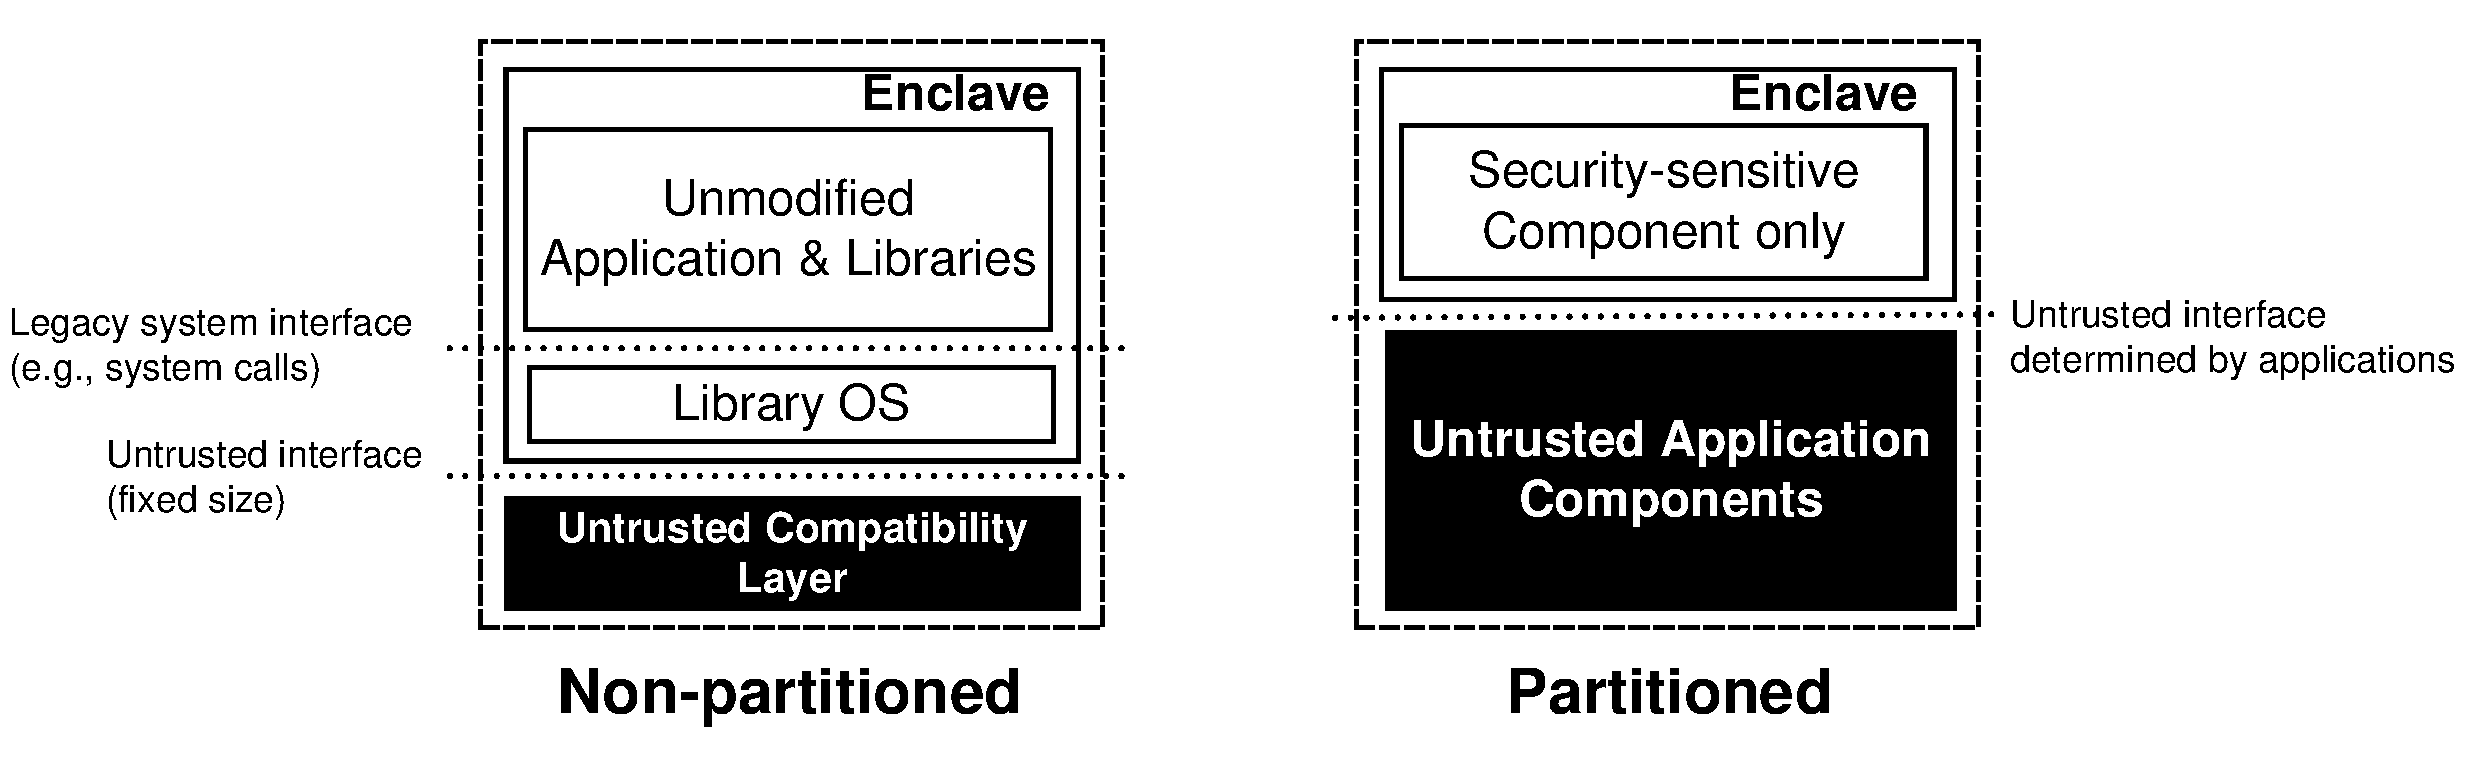
\includegraphics[width=\linewidth]{figures/libosvssdk.pdf}
%\footnotesize
%\vspace{-0.3in}
%\caption{
%Comparison between libOS-based model (e.g., \haven{} and \graphenesgx{})
%and SDK-based (SDK for \sgx{}) model for migrating applications in enclaves.
%Green (light) boxes are trusted components and red (dark) boxes are untrusted.
%The libOS-based model often yields a larger TCB in the enclave,
%while the SDK-based model requires developers to be responsible of
%securing the enclave on the untrusted interface.
%}
%\label{fig:libosvssdk}
%\end{figure}




%%% \sgx{} is a new feature on the 6th-genaration \intel{} CPUs.
%%% it contains a set of new x86/64 instructions, to initiate, destroy, and attest isolated execution environments (i.e., enclaves) in the address space of applications.
%%% When \sgx{} loads an application in an enclave,
%%% the code and data of the application will remain encrypted in the main memory,
%%% forbidding any mean to eavesdrop the application secrets.
%is a set of new x86/x64 instructions introduced
%to the latest \intel{} CPUs,
%to bootstrap an isolated execution environment
%inside applications' virtual memory address space.
%\sgx{} creates a memory region
%(generally referred as {\bf enclave}), storing both the code and data of the isolated execution,
%which stays encrypted in DRAMs and only the CPU is capable of encryption and decryption.
%The CPU derives the encryption key
%from the cryptographic measurement of the initial state of enclave memory,
%to allow remote entities to verify the soundness of execution and establish the trust
%needed for provisioning sensitive data.

SGX enables the defense against a threat model where one only trusts the Intel CPUs and the 
code running in the enclaves.
%whereas the rest of application, system software, off-CPU-package hardware devices and providers are untrusted. 
SGX protects applications from three different types of attacks on the same host, which are summarized in Figure~\ref{fig:sgx:threats}. First, untrusted application code inside the same process but outside the enclave
cannot access enclave memory or arbitrarily jump into enclave code. Second, OSes, hypervisors, and other system software cannot peek into enclaves from administrative domains;
%\fixme{added Mona's suggestion}
Third, other applications on the same host
cannot exploit vulnerabilities in a OS kernel or system software
to escalate privileges.
Finally, off-chip hardware, such as buses, DRAM, and peripheral devices can be hijacked or replaced with malicious components, but can never steal or corrupt enclave secrets
both encrypted and authenticated inside the memory. 
A SGX enclave can choose to trust a remote service or enclave and be trusted in return
after performing a procedure of inter-platform attestation~\cite{sgx-attestation}.


\begin{figure}[t!]
\centering
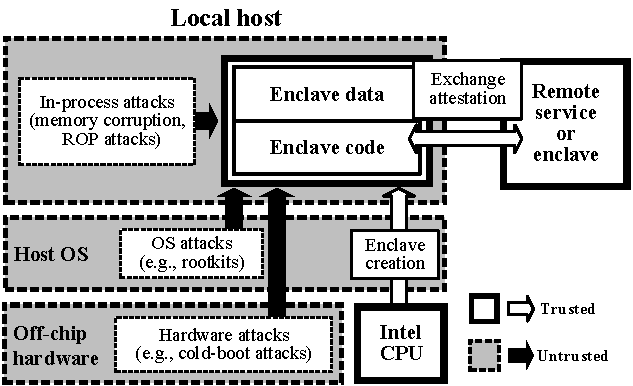
\includegraphics[width=\linewidth]{sgx.pdf}
\caption{The threat model of SGX. SGX protects applications
from three types of attacks:
in-process attacks from outside of the enclave,
attacks from OS or hypervisor, and attacks from off-chip hardware.}
% Red (dark) boxes are untrusted components and green (light) boxes are trusted.}
%For each enclave, \sgx{} establishes the chain of trust from the \intel{} CPU.
%Enclaves across physical machines or even infrastructures can remotely attest the integrity of execution, using the signatures generated and signed by the CPU.
%Green (light) boxes and arrows represent the trusted components and operations, and red (dark) boxes and arrows represent the otherwise.
\label{fig:sgx:threats}
\end{figure}



%%% \begin{compactenum}

%%% \item {\bf Inside process memory:}
%%% \sgx{} partitions the application process into two privilege levels, as the trusted part (in enclaves) which can access the whole process memory, and the untrusted part (outside enclaves) forbidden to access enclave memory.
%%% %the privileged part (in the  enclave region) can access all process memory,
%%% %while the unprivileged part (outside the enclave region) is limited to access only data that are not isolated by \sgx{}.

%%% \item {\bf From hosting OSes or hypervisors:}
%%% \sgx{} assumes that OSes and hypervisors can be compromised by either exploiting system vulnerabilities
%%% or malicious system software installed by administrators.
%%% Both types of compromise are legitimate threats to modern OSes, due to complexity of modern OSes and usage of public facilities like clouds.

%%% %Operating systems or hypervisors
%%% %that are either compromised by rootkits
%%% %or deliberately modified by the host providers.
%%% %An attacking host can access the raw data in DRAMs, or remap the
%%% %physical pages to other contexts.

%%% \item {\bf Physically from the hardware:}
%%% One type of attacks that cannot be defended by software-based solutions~\cite{flicker, criswell2014virtualghost}
%%% is from the attackers who have physical access to the hosts.
%%% \sgx{} can resist attacks on the host hardware
%%% including hacking peripheral devices like ethernet cards and connectors~\cite{hudson15thunderstrike}, tapping into buses, or eavesdroping DRAM data using Cold-boot attack~\cite{halderman09coldboot}.


%%% \end{compactenum}


%%% \sgx{} protects an application against unpredictable threats from both local and remote hosts.
%%% \sgx{} establishes a trusted path
%%% from one enclave to another,
%%% providing end-to-end protection to both enclaves to
%%% exchange data with confidentiality and integrity.
%%% %, processing the data and returning the computation results with end-to-end protection.
%%% We can further divide up the protection using \sgx{} into three elements:
%The use cases of \sgx{} mostly involve the process that an enclave
%retrieves a signed attestation from the processor,
%to exchange provisioning of critical information from remote servers.
%The purpose of such process is equivalent to
%expanding the trusted execution
%from remote servers
%to untrusted hosts,
%to harness resources such as CPU cycles and DRAMs.

%%% \begin{compactenum}

%%% \item {\bf Isolated execution:}
%%% \sgx{} guarantees the execution initiated in an enclave
%%% to be isolated from any part of the system except the enclave itself.
%%% %any part of the system except the enclave itself can access the execution state. 
%%% Achieved by the secrecy of encryption keys in \intel{} CPUs.

%%% \item {\bf Attestation of integrity:}
%%% Remote entities with a \sgx{}-enabled CPU can verify the integrity of an enclave, using the \intel{} Attestation Services (ISV)~\cite{isv}.
%%% %for its integrity of running the exact code that it is given.
%%% Achieved by the uniqueness of CPU keys to sign the cryptographic measurement of enclaves.

%%% \item {\bf Authentication:}
%%% Remote entities can identify the owners of enclaves by distinguishing the cryptographic measurements generated with different signing keys.


%%% %explicitly launched for processing the specific tasks, regardless of the identicality of execution.
%%% %That is, two mutually distrusting users can launch the same execution in  separate enclaves, yet be able to distinguish by the measurements as MACs (Message Authentication Code) signed by the users' private keys.

%%% \end{compactenum}


%One must note that \sgx{} only promises the integrity of application binaries
%initially loaded in enclaves.
%The gap between integrity of binaries and complete security has to be filled
%by ones who develop and approve the applications.
%More specifically, the clients are responsible of
%testing whether the applications contain any vulnerabilities
%that lead to information leak.
%To minimize the risk of leaving any flaws in the applications unintentionally,
%developers often tend to cut down the trusted computing base (TCB)
%of the applications. With smaller TCB, clients who launched the enclaves
%can more easily reason about the thoroughness of securing the execution.

%To achieve smaller TCB, the software development kit of \sgx{}
%intends to encourage developers to partition the applications and
%keep only security sensitive components in the enclaves.
%Such an intention is exactly contradicted by the trust model of \haven{},
%which must trust the loaded application as a whole.
%Except for the cases in which the whole applications must be secured,
%\haven{} actually downgrades the trustworthiness of enclaves.
%Figure~\ref{fig:libosvssdk} shows the comparison of the two models.


%%% By synthesizing and streamlining these three elements (i.e., isolation, attestation and authentication),
%%% \sgx{} provides a promising build block to securing applications
%%% from unpreditable security threats.

%developing applications
%that are resistant to unpreditable, unavoidable threats.
%Users expect \sgx{} to build up a wall for protecting the sensitive data, even against a catastrophic scenario like a complete takeover of the infrastructure.  

%\fixmedp{Explain how to read the figures in the captions. What do colors and shading mean?}
%
%\fixme{Disabled the whole discussion about SDK. dp: ok with me, but probably drop from figure} 
\begin{comment}
\subsection{The legacy framework (The \sdk{})}

{\bf Intel's \sgx{} SDK} (software development kit) for Linux~\cite{intel-sgx-sdk} is the official framework
for programming \sgx{} execution within Linux applications.
\sdk{} includes the components of two phases:
a {\bf compile-time utility} to generate a valid executable for running inside enclave,
and a {\bf run-time framework} to trigger the hardware-enforced isolated execution.
The two-phased design is based on the assumption that compilation of applications
is controlled by trusted, security experts,
to retain the trustworthiness of isolation model when running on untrusted OSes.


The work flow of \sgx{} programming using \sdk{} is as follows:
\begin{compactenum}
\item At the build-time (on trusted hosts), developers create a self-contained, static executable as the initial code and data after enclave creation.
We refer the executable as an ``enclave image''.
The enclave image is statically links with the enclave infrastructure, which provides enclave APIs (e.g., retrieving attestation) and a extremely small set of POSIX functions (e.g., {\tt memset()}).
After linking, the compile-time utility signs the executable and inserts the enclave signature structure
({\tt SIGSTRUCT}) in the application code.
\item At the execution-time (on untrusted hosts), the enclave image is taken by the framework. The user-space driver then requests enclave creation with the kernel driver, through {\tt ioctl()} to a pseudo-device {\tt /dev/isgx}.
The kernel driver creates and initializes an enclave using the authenticated signature structure,
and a token exchanged from an architectural enclave, {\tt AESMD}, for ensuring the validity of enclave. 
\end{compactenum}





%During the compile time,
%the developers create a self-contained, static binary, as the initial image of an run-time enclave (an ``enclave image'').
%\sdk{} provides the infrastructural libraries (libsgx) for static linking, which contain enclave APIs and few POSIX functions.
%A signing tool of \sdk{} will generates a valid enclave signature
%derived from the enclave image.
%Both the static linking and signing must happen on a trusted, development machine.


%After generating the enclave image, developers then ship it with the rest of application,
%to untrusted hosts (\sgx{}-enabled)
%where the \sdk{} run-time framework is installed.
%The run-time framework provides both kernel and user-space drivers,
%to interface \sgx{} hardware using the new x86 instructions (e.g., {\tt ECREATE}, {\tt EADD}, {\tt EENTER}).
%The framework also includes an architectural enclave (AESM), for validating the enclave attributes (and generating a run-time token),
%and a kernel EPC (enclave page cache) driver that manages paging for all running enclaves.



% includes both compile-time and run-time components:
%for the compile time, the SDK provides all the infrastructure libraries,
%which the applications statically link with,
%and a signing tool that generates the enclave signatures for hardware validation.
%The run-time framework then takes the signed enclave binaries,
%and uses the kernel and user-space drivers to initiate the isolated execution in enclaves.



\sdk{} centers the whole programming model based on the concept of partitioning an application,
and isolating only minimum application code in enclaves.
The partitioning minimizes the risk of compromising the enclaves,
due to smaller trusted computing base (TCB) and less opportunity of omitting security glitches.
With this model,
developers are expected
to identify the part of an application that performs the sensitive operations,
and define an validated interface to
the sensitive part and rest of the application.
\sdk{} encourages partitioning by reducing the difficulty of defining and accessing the interface---a language tool automatically generates the interface code with extra argument-sanitizing code.
The generated interface code essentially filters input and output of the enclave,
and prevents randomly copying memory across the enclave boundary, leaking or corrupting internal data.


%The Intel SDK has its limitations. The infrastructure of the SDK provides APIs in enclaves for accessing SGX features (e.g., attestation), as well as a small set of POSIX APIs
%(\roughly{}10 functions, such as {\tt printf} and {\tt memset}).


Despite that \sdk{} attempts to alleviate the difficulty of partitioning for SGX,
porting a piece of application code that is sophisticated and interactive to the rest of application
is still a significant cost to pay.
In general, developers want to find a reasonable granularity of partitioning---a ``sweet spot'' that partitions the application code neither too small nor too large, 
to nicely balance between frequency of enclave exits and risk of introducing incompatible code.
For an application written in C/C++, partitioning is cumbersome especially if the application is poorly modularized.


Unfortunately, the limited POSIX support in the \sdk{} infrastructure really strikes
the opportunity of fine-grained partitioning.
The lack of POSIX APIs in the infrastructure is fundamental, due to the restriction
on OS interaction from the enclaves.
The missing APIs encapsulates system calls, which can expose the enclave to some risky OS interaction model, such as {\bf Iago Attacks}~\cite{checkoway13iago}.

%In conclusion, this work targets on completing the API support, either at POSIX level or system calls,
%while retaining the isolation model.
%The platform can assist developers to refocus on partitioning applications for minimizing the risks.

\end{comment}

\subsection{SGX frameworks}
\label{sec:sgx:background:design}



%This subsection summarizes the principal design choices facing any 
%framework for running applications on SGX.  We explain the decisions in
%recent systems for SGX applications, and the trade-offs in this space.

\issuedone{1.2.c}{compare library OS approach with shim layers}
Despite the security benefits,
%Unfortunately, applications do not ``just work'' on SGX.
SGX imposes a number of restrictions on enclave code 
that require application changes
or a layer of indirection. % to work around.
Some of these restrictions are motivated by security, such as disallowing system calls
inside of an enclave, so that system call results can be sanitized by a piece of carefully-written shielding code in the enclave before being used by the application.
%Other restrictions are subtle interactions with unrelated other features, such
%as disallowing the {\tt cpuid} instruction to ensure clear semantics when SGX is combined
%with VT (one mode of VT ensures that using {\tt cpuid} will trap to the hypervisor).
%Intel's SGX SDK includes a limited C library, which is missing a number of features by design.
The typical applications
for processing security-sensitive data
in a cloud environment
include servers, language runtimes, and
command-line programs,
%databases (not all are evaluated in this paper), 
which rely on faithful emulation of Linux system call semantics, such as \syscall{mmap} and \syscall{futex}.
Developers who wish to run these applications on SGX
must either use 
a trusted, wrapper library that reproduces these semantics in an enclave, or replace large portion of application code
unrelated to security.
The extra effort for adapting existing application code
into SGX causes delay to deployment of the technology; a number of \fixme{cite some examples here} security-sensitive applications
can benefit from porting into SGX as soon as possible.




%Besides SGX, a number of CPU vendors are developing similar, but not identical, hardware protection mechanisms, including IBM's SecureBlue++~\cite{secureblue++} and AMD SEV~\cite{amd-sme}---each
%with different idiosyncrasies.
%Thus, the need to adapt applications to use hardware security features will only increase in the near term.


Related work shows concerns about the significant code changes to applications involved during porting to SGX.
Although Haven~\cite{baumann14haven} showed that a library OS
could run unmodified applications on SGX, this work pre-dated availability of SGX hardware.
Since then, several papers have argued that the library OS approach is impractical for SGX,
both in performance overhead and trusted computing base (TCB) bloat, and that one must instead refactor one's application for SGX.
For instance, a feasibility analysis in the \scone{} paper
concludes that ``On average, the library OS increases the TCB size by $5\times$, the service latency by $4\times$,
and halves the service throughput''~\cite{osdi16scone}.
Shinde et al.~\cite{shinde17panoply} argue that using a library OS, including libc, increases TCB size by two orders of magnitude over
a thin API wrapper layer with shielding ability, called \panoply{}.




\graphenesgx{} shows that 
a \libos{} can facilitate deployment of an unmodified application to SGX,
granting immediate security benefits
without crippling performance cost and full-blown TCB increase.
The comparison between \liboses{} and thin shielding layers is inclusive in many ways.
Besides the fact that
Haven is evaluated upon a simulated hardware,
Haven has a large TCB due to using Drawbridge~\cite{porter11drawbridge},
a full-featured \libos{}
which recycles a significant portion of the Windows 7 source code.
\graphenesgx{}, on the other hand,
shows performance overheads comparable to the range of overheads reported in \scone{} and \panoply{}.
The initial publication of \panoply{} also notes that \graphenesgx{}
is 5-10\% faster than \panoply{}~\cite{shinde17panoply}.
Arguments about TCB size are more nuanced, and a significant amount of the discrepancies
arise when comparing incidental choices like \libc{} implementation (e.g., musl vs.\ \glibc{}).
\graphene{}, not including \glibc{}, adds 53 kLoC to the application's TCB, which is comparable to
\panoply{}'s 20 kLoC or \scone{}'s 97 kLoC. % 
Our position is that the primary reduction to TCB comes from either compiling out
unused library functionality, as in a unikernel~\cite{unikernels}.% and measured by our prior work~\cite{tsai16apistudy};
or further partitioning an application into multiple enclaves with fewer
OS requirements.
%, such as just
%terminating a TLS connection in the enclave.
When one normalizes for functionality required by the code in the enclave, the design choice between a library OS or a thin shielding layer has no significant impact on TCB size.

%To be clear, SGX-specific coding has benefits, but we must not let the perfect be the enemy of the good.
%For example, privilege separating a complex application into multiple enclaves may be a good idea
%for security~\cite{flicker,Provos:2003:PPE:1251353.1251369,shinde17panoply}, and replacing particularly expensive operations can improve performance on SGX.
%%Our experience with supporting a rich array of applications on SGX, including web servers, language runtimes, and
%%databases (not all are evaluated in this paper), is that
%%a number of software components orthogonal to the primary functionality of the application
%%rely on faithful emulation of arcane semantics of Linux system calls, such as {\tt mmap} and {\tt futex}.
%The goal of \graphene{} is to bring up rich applications on SGX quickly, and then let developers
%optimize code or reduce the TCB as needed.


Besides running unmodified Linux binaries on SGX, \graphenesgx{} also contributes a number of usability enhancements,
including integrity support for dynamically-loaded libraries, enclave-level forking, and secure inter-process communication (IPC).
Users need only configure features and cryptographically sign the configuration.
\graphenesgx{} is also useful as a tool to accelerate SGX research.
%\graphenesgx{} has been open-sourced since June 2016\footnote{Available at https://github.com/oscarlab/graphene}.
\graphenesgx{} does not subvert
any opportunities of optimizing an application for SGX or partitioning application code outside of an enclave for further reducing TCB size.
A number of SGX frameworks and security enhancements~\cite{orenbach17eleos,kuvaiskii17sgxbound,shih2017t-sgx,seo2017sgx-shield} present techniques that are complementary to \graphenesgx{}. 

%Although our focus is unmodified applications, \graphenesgx{} can also run smaller pieces of
%code in an enclave, as in a partitioned application.
%Several papers already compared against or extended 
%\graphenesgx{}~\cite{shinde17panoply, orenbach17eleos, kim2017enhancing}
%\fixmedp{I think there are more - Chia-Che please check recent google scholar activity}\fixme{these are all I can find; others are all just citing Graphene as related work}, 
%and we are aware of ongoing projects using \graphenesgx{}.
%One published paper has already benchmarked against Graphene-SGX~\cite{shinde17panoply},
%and we are aware of a number of concurrent submissions to other conferences that
%use Graphene as either a building block or comparison point for software that uses SGX.
%In a short time, Graphene-SGX has already had significant use outside of this group,
%Has already been benchmarked in published papers by other groups.
%We are aware of several concurrent submissions to other conferences that are
%buiding extensions to Graphene


\subsection{Shielding complexity}


\paragraph{How much functionality to pull into the enclave?}
At one extreme, a library OS like Haven~\cite{baumann14haven} pulls most
of the application-supporting code of the OS into the enclave.
On the other extreme, thin ``shim'' layers, like \scone{}~\cite{osdi16scone} and \panoply{}~\cite{shinde17panoply} 
wrap an API layer such as the system call table.
Pulling more code into the enclave increases the size of the TCB,
but can reduce the size and complexity of the interface, and attack surface, 
between the enclave
and the untrusted OS.

The impact of this choice on performance
largely depends on two issues. First, entering or exiting the enclave 
is expensive; if the division of labor reduces enclave border crossings, 
it will improve performance.
The second is the size of the Enclave Page Cache (EPC),
limited to 128MB on version 1 of SGX.
If a large supporting framework tips the application's working set size
past this mark, the enclave will incur expensive swapping.


\paragraph{Shielding complexity.}
\issue{1.2.f}{Clarify the details about Iago attacks}
SGX hardware can isolate an application from an untrusted OS, but 
SGX alone can't protect an application that  requires
functionality from the OS.  {\em Iago attacks}~\cite{checkoway13iago}
are semantic attacks from the untrusted OS against the application, where an unchecked system call return 
value or effect compromises the application.
Iago attacks can be subtle and hard to comprehensively detect, at least with the current
POSIX or Linux system call table interfaces.

Thus, any SGX framework must provide some {\em shielding} support, to 
validate or reject inputs from the untrusted OS.  
The complexity of shielding is directly related to the interface complexity:
inasmuch as a library OS or shim can reduce the size or complexity of the 
enclave API, 
the risks of a successful Iago attack are reduced.

\paragraph{Application code complexity.}
Common example applications for SGX in the literature 
amount to a simple network service running a TLS
library in the enclave, putting minimal demands on a shim layer. 
Even modestly complex applications, such as the R runtime and a simple
analytics package, require dozens of system calls providing wide-ranging functionality, 
including \syscall{fork} and \syscall{execve}.
For these applications, the options for the user or developer become: 
(1) modifying the application to require less of the runtime; (2) opening and shielding more 
interfaces to the untrusted OS; (3) pulling more functionality into a shim or a library OS.
The goal of this paper is to provide an efficient baseline, based on (3),
so that users can quickly run applications on SGX, and developers can 
explore (1) or (2) at their leisure.

\paragraph{Application partitioning.} An application can have multiple
enclaves, or put less important functionality outside of the enclave.
For instance, a web server can keep cryptographic keys in an enclave,
but still allow client requests to be serviced outside of the enclave.
Similarly, a privilege-separated or multi-principal application might create a separate enclave for
each privilege level.

This level of analysis is application-specific, and beyond the focus of this paper.
%which is on running unmodified applications in enclaves.
However, partitioning a complex application into multiple enclaves
can be good for security. In support of this goal,
\graphenesgx{} can run smaller pieces of code, such as a library, in an enclave, as well as
coordinate shared state across enclaves.

%* Partitioned vs. unpartitioned app?

%** Right choice depends a lot on whether the app has multiple principals or security concerns.

\begin{comment}
\fixmedp{Did a first cut at 2.2; needs to integrate the figure (or drop it).  I didn't know what to write for 2.3 yet.  I left the old text below for now (if there is anything you really want to save), but it needs to go away}

\subsection{Open Challenges}

\fixmedp{Here, I would give a taste of some of the issues we solve and why they are hard, like dynamic loading (and maybe fork or IPC).  Keep it short, a few paragraphs.}
\end{comment}

%\begin{figure}[t!]
%\centering
%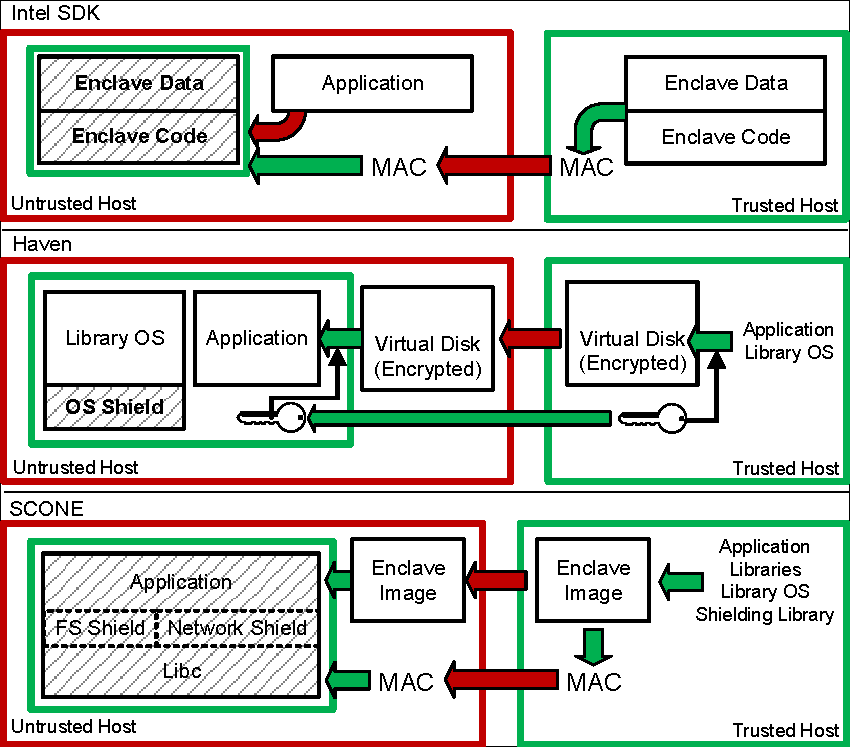
\includegraphics[width=\linewidth]{figures/sdkvslibos.pdf}
%\caption{Comparison of the code integrity model among different \sgx{} frameworks, including the \sdk{}, \haven{} and \scone{}.}
%%Green (light) boxes and arrows represent the trusted components
%%and operations, and red (dark) boxes and arrows represent the otherwise.
%%Patterned blocks represent the code and data included in the initial measurements of the enclaves.}
%\label{fig:sdkvslibos}
%\end{figure}


\begin{comment}
\subsection{\sgx{} shielding systems}
\label{sec:background:shielding-systems}




The current \sgx{} shielding systems, such as \haven{}~\cite{baumann14haven}, \scone{}~\cite{osdi16scone}, and Panoply~\cite{shinde17panoply}, enforce end-to-end isolation to
legacy applications without partitioning.
A \sgx{} shielding system preserves the trusted computing base (TCB)
of an application, and further increases it with a shielding layer to defend against the untrusted OSes.
By avoiding application partitioning,
%model of quarantining an unmodified, COTS application in an \sgx{} enclave.
a shielding system minimizes the effort of reprogramming the applications for \sgx{} execution, often with recompilation or packaging the binaries in an encrypted enclave.
%to merely recompiling or packaging the application code before signing it off for enclave execution.
%These \libos{}es internalize OS features into the enclave, to maintain a fixed-size,
%narrow interface to the untrusted host OSes.
%Porting applications using a \sgx{} \libos{} is vastly different from the programming model of \sdk{}---no programming effort is needed when porting with a \sgx{} \libos{}, and applications are isolated without partitioning.
In the following paragraphs, we compare the current shielding systems with the \graphenesgx{} approach.

\haven{}~\cite{baumann14haven} uses a \libos{} called \drawbridge{} in each enclave
to shield a single-process \emph{Windows} application from the untrusted host OS.
\haven{} absorbs the implementation of system APIs (i.e., Win32 APIs) from the host OS,
%\haven{} uses \drawbridge{}~\cite{porter11drawbridge} as the backbone of its enclave infrastructure, 
and exports a narrow enclave interface on which untrusted inputs are carefully filtered to defend against the Iago-type attacks.
Adding a \libos{} to each enclave causes a bloat of TCB---for \haven{}, the size of a \libos{} binary and shielding layer is \roughly{}200MB.
\haven{} has to establish the trust and integrity in all these binaries loaded into an enclave. Except that the shielding layer is a part of the enclave since its creation, \haven{} enforces the integrity of both the \libos{} and the isolated application,
by storing all binaries on an encrypted virtual disk and relying a remote, trusted server to provision the key for decryption.
\haven{} builds a trusted path from a remote server to local cloud machines,
to securely bootstrap application execution inside the enclaves.
%Other minor comparison between \haven{} and this work: the development and evaluation of \haven{}, at publication, is based on a simulated architecture.
%On the contrast, \graphenesgx{} is a released open-source platform, tested by many developers from institutes and corporations. \fixme{maybe bring up TCB?}



\scone{}~\cite{osdi16scone} isolates Linux micro-services in enclaves as a container-like environment.
After a brief attempt of building a \libos{} like \haven{},
\scone{} chooses a different approach of shielding the system API usage in applications, by designing shielding strategies based on each API.
\scone{} stacks the application on top of file-system and network shielding libraries, and extends a standard library C (musl~\cite{musl}) to securely exit the enclave for system calls.
Within the \sgx{}-aware Libc, \scone{} carefully filters the inputs from the host system calls, as the defend against known Iago attacks.
For instance, \scone{} ensures that pointers given to and returned by a host system call will point to addresses outside the enclave,
to prevent the host OS to manipulate pointers and cause memory corruption in the enclave.
\scone{} also authenticates or encrypts file or network streams
based on configurations given by the developers.


%The \libos{} implementation in \scone{} is based on musl~\cite{musl} and LKL (Linux kernel library)~\cite{lkl}.
%The design of a SCONE enclave (or Secure Container) has similarity
%with a basic block of \graphenesgx{}:
%they both validate input files based on cryptographic methods, and are fully configurable at a per-file basis.
%However, \graphenesgx{} supports a more complete set of Linux system APIs.
%The APIs that \graphenesgx{} especially contributes over \scone{} are the Linux multi-process APIs, including copy-on-write {\tt fork()}, {\tt exec()}, signals, and system V IPC (message queues and semaphores).

Panoply~\cite{shinde17panoply} further reduces the TCB of a shielding system over the SCONE approach, by excluding both a \libos{} and \libc{} from enclaves.
Instead, Panoply uses a shim layer shielding a portion of the POSIX API. The shim layer yields about 20 KLoC as its TCB (trusted computing base), which is much smaller than libc and/or a library OS.
% in other shielding systems.
As Panoply delegates the libc functions outside the enclave, its shim library defends the supported POSIX API,
including 91 {\em safe} functions and 163 {\em wild (unsafe)} functions.
Panoply also supports multi-process API including \fork{}, \exec{}, signaling, and sharing untrusted memory with inline encryption.
Compared to \graphenesgx{}, Panoply has made some different design decisions in supporting multi-process API,
including supporting fork by copying memory on-demand with statically determining memory access,
and using secured messaging for inter-process negotiating instead of coordinating over an encrypted RPC stream.




\subsection{Comparison and security implications}

\fixme{need to drop the SDK discussion, revisit the security claims, and discuss Iago attacks in details.}

Figure~\ref{fig:sdkvslibos} shows the comparison between \haven{}, \scone{}, Panoply, and \graphenesgx{}.
%The \sdk{} model uses a static MAC of the enclave code and data, given to the \sgx{} driver for bootstrapping the isolated execution.
The \haven{} model only initiates enclaves with the OS shield layer,
which unpacks the enclave binaries from a virtual disk---decrypted using a provisioned key.  
The \scone{} model extends the \sdk{} model---it statically links the application binaries with the shielding library, creating a static enclave image verifiable by its MAC. The \sdk{} and \scone{} model retain more flexibility in deploying and integrating \sgx{} enclaves by focusing on the code integrity rather than encryption.

The key concerns that affects users choosing among these solutions are {\bf trusted computing base (TCB) size} and {\bf attack surface}.
However, since all these solutions are based on different design decisions, assumption and requirements, the comparison of TCB size and attack surface is often imprecise and inconclusive.

\paragraph{TCB size.}
Most studies measure the TCB size of a system by the total LoC (lines of code) written for all the trusted components, or the size (in bytes) of all the trusted binaries.
The comparison of TCB size is only meaningful when two systems have comparable system features,
and are order-of-magnitude different in term of LoC or binary size.
For instance, the comparison of TCB size between \haven{} and \scone{} is never an apples-to-apples comparison.
The implemented system features and personalities
in these two systems are fundamentally different, and \haven{} supports a much larger fraction of Windows features than the fraction of Linux features supported by \scone{}.

We argue that the only occasion that the reduction of TCB size
can be convincingly demonstrated is when a design has partitioned a system into isolated components,
or removed unreachable execution paths.
For instance, the \sdk{} promotes application partitioning for \sgx{};
it requires additional partitioning effort but is effective for confining the TCB size.
By statically linking the application binaries
with the shielding layers and standard C library, \scone{} offers more opportunities in stripping the Libc and shield code of unused APIs, and thus reducing its TCB size.



\paragraph{Attack surface.}

Most studies estimate the severity of having an attack surface by the size of interface to the trusted and untrusted components.
The experience of \scone{} provides an important insight for estimating attack surface: the narrowness of interface is not proportional to the difficulty of defending against incoming attacks.
An interface overloaded with too many features or semantics can become a major source of vulnerabilities.

%\subsection{The \graphene{} Library OS}
%
%\graphene{}~\cite{tsai14graphene} introduces a \libos{} design that supports
%both single-process and multi-process Linux applications,
%but retains a narrow host interface (43 functions) as a vantage point for enforcing security isolation.
%The main contribution of \graphene{} is an distributed implementation of the POSIX namespace coordination,
%to support Linux multi-process abstractions across \libos{} instances.
%All the multi-process abstractions in \graphene{} is implemented using simple pipe-like RPC streams,
%without relying on any host memory sharing support.
%Based on this design, \graphene{} can easily isolate mutually untrusting applications,
%by blocking the RPC streams between unrelated applications.
%
%
%
%The design decisions made by \graphene{} are important keys to the \graphenesgx{} framework.
%First, the host interface contains mostly internal abstractions, and three external ones including files, network connections, and RPC streams.
%The simplicity of the host interface facilitates shielding the \libos{}
%from risky OS interaction.
%Moreover, \graphene{} implements multi-process abstractions across instances without memory sharing.
%\graphenesgx{} can rely on the distributed POSIX implementation
%to support multi-process applications across multiple enclaves, by coordination over validated RPC streams.


\end{comment}



